% Sección del artículo — dueño: P3.
\section{Metodología}
\subsection{Simulador, condiciones y datos}
\textbf{Mundo.} Cada escenario es un área de $60\times60$\,m discretizada a 0.5\,m con una
base, tres a cinco puntos de inspección y obstáculos circulares y rectangulares. Una parte de
los obstáculos figura en el \emph{mapa previo} que conoce el dron; el resto no está previsto.
Se generan seis condiciones (Fig.~\ref{fig:escenarios}): nominal, obstáculos no previstos,
obstáculos móviles, viento con ráfagas, pérdida de GPS tras visitar el último punto, y
combinada. El paso de simulación es de 1\,s, el dron se mueve 0.8\,m por paso y choca si la
distancia libre es menor que su radio; el viento se suma al desplazamiento comandado.

\textbf{Sensores.} El dron percibe (Fig.~\ref{fig:sensores}): (i) el \emph{ojo de la mosca},
un parche de ocupación egocéntrico de $32\times32$ alineado con el rumbo; (ii) 32 rayos de
distancia de hasta 8\,m, que usa sólo el supervisor; (iii) la \emph{panorámica de la abeja},
72 sectores de 5\textdegree{} alineados con la brújula, con la elevación aparente de los
objetos visibles; y (iv) brújula, odometría (ciega al viento, por eso deriva) y GPS ruidoso
mientras esté disponible. Son abstracciones deliberadas de una cámara de eventos o un sensor
de profundidad, de un anillo ToF y de una cámara omnidireccional de baja resolución.

\textbf{Por qué 2.5D.} El dron vuela a altura fija y el vector a casa es horizontal, como en
el trabajo de Firlefyn et~al., que fijan el cuadricóptero a 1.89\,m~\cite{firlefyn2024}; por
eso el movimiento se simula en el plano. La percepción de la abeja, en cambio, no es plana:
cada objeto tiene altura y el sensor registra su elevación angular $\arctan(h/d)$, con
oclusiones (en cada sector domina el objeto más alto), es decir, la silueta del horizonte que
usan los insectos para orientarse.

\textbf{Validación del sensor.} Antes de entrenar se comprobó, en
\nfbIdfEscenarios{} escenarios de prueba, que la silueta reproduce tres propiedades conocidas
de los panoramas reales (Fig.~\ref{fig:sensor}). (i) La función de diferencia de imagen
(IDF)~\cite{zeil2003}, la diferencia RMS con la vista de casa, crece de forma monótona con la
distancia (correlación de Spearman media \nfbIdfSpearman{}; monótona en el \nfbIdfMonotonas{}
de los escenarios) y supera el umbral de llegada del ALV a \nfbIdfRadioLlegada{}\,m de la
base, por encima del piso que deja el ruido (\nfbIdfPisoRuido{}). (ii) Girar el panorama y
buscar el mínimo de la IDF rotacional recupera el rumbo con un error mediano de
\nfbRumboErrorDos{} a 2\,m y \nfbRumboErrorCuatro{} a 4\,m. (iii) El ALV apunta a casa con
error menor de 90\textdegree{} (condición para acercarse) en el \nfbAlvCaptura{} del entorno.
El sensor no modela textura, iluminación, la inclinación del dron por el viento ni la altura
del ojo; son limitaciones declaradas en la Sec.~\ref{sec:discusion}.


\textbf{Particiones sin fuga.} Cada escenario se genera de forma determinista a partir de su
semilla: entrenamiento usa las semillas 0--9\,999, validación 10\,000--10\,999 y prueba
20\,000--20\,999. La validación se usa para elegir la mejor época y la prueba sólo para el
informe final; una prueba automática verifica que los rangos no se solapan. Como cada semilla
es un mundo distinto, la prueba se hace sobre mundos que ninguna red vio.

\textbf{Experto y datos.} Un experto con información privilegiada (mapa completo y posición
real, que el dron nunca tiene) planifica con A* y descarta maniobras que acerquen a un
obstáculo móvil en el horizonte de predicción; resuelve el \nfbExitoExperto{} de
\nfbEpisodiosExperto{} misiones de validación. Sus decisiones en
\nfbEpisodiosMoscaTrain{} episodios de entrenamiento dan \nfbMuestrasMoscaTrain{} muestras para
la mosca, y para la abeja se muestrean pares (vista actual, vista memorizada) con la dirección
y distancia reales a la base (Tabla~\ref{tab:datos}). Las acciones están desbalanceadas:
\emph{avanzar} es el \nfbPctAvanzar{} de las muestras y \emph{mantener posición} sólo el
\nfbPctMantener{}.

\begin{table}[t]
\caption{Conjuntos de datos generados por el experto}\label{tab:datos}
\centering
\resizebox{\linewidth}{!}{%
\begin{tabular}{lrrrr}
\toprule
 & \multicolumn{2}{c}{Mosca} & \multicolumn{2}{c}{Abeja} \\
Partición & Episodios & Muestras & Escenarios & Pares \\
\midrule
Entrenamiento & \nfbEpisodiosMoscaTrain & \nfbMuestrasMoscaTrain & \nfbEpisodiosAbejaTrain & \nfbMuestrasAbejaTrain \\
Validación & \nfbEpisodiosMoscaVal & \nfbMuestrasMoscaVal & \nfbEpisodiosAbejaVal & \nfbMuestrasAbejaVal \\
Prueba & \multicolumn{2}{c}{lazo cerrado: \nfbEpisodiosPorCondicion{} por condición} & \nfbEpisodiosAbejaTest & \nfbMuestrasAbejaTest \\
\bottomrule
\end{tabular}}
\end{table}

\begin{figure*}[t]
\centering
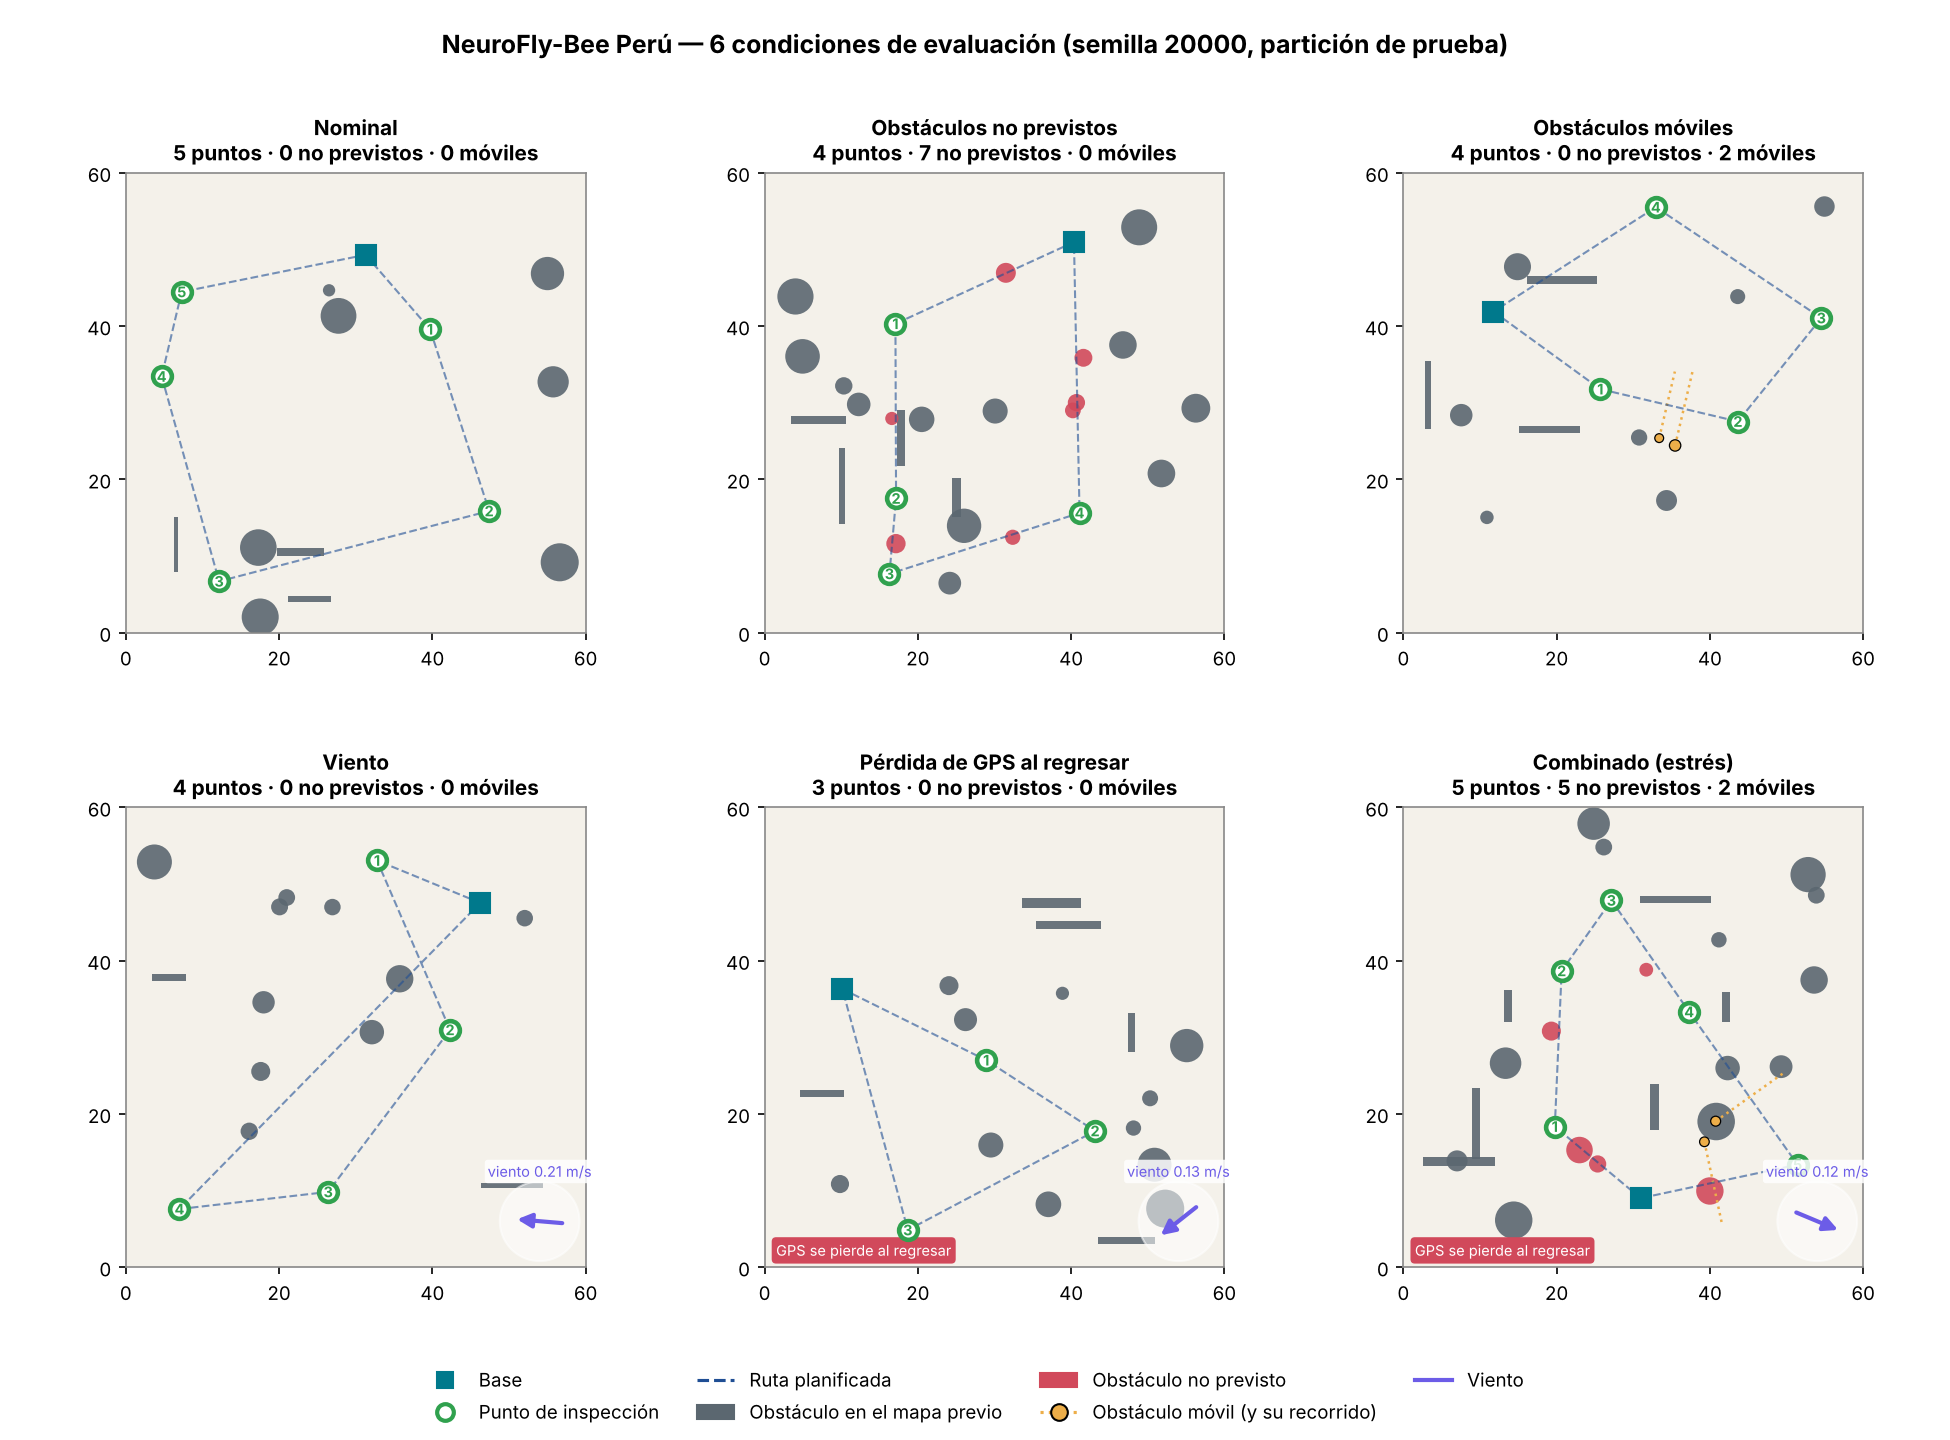
\includegraphics[width=0.85\textwidth]{v3_escenarios}
\caption{Las seis condiciones para una misma semilla de prueba. Gris: obstáculos del mapa
previo; rojo: no previstos; naranja: móviles con su recorrido; verde: puntos de inspección.}
\label{fig:escenarios}
\end{figure*}

\begin{figure*}[t]
\centering
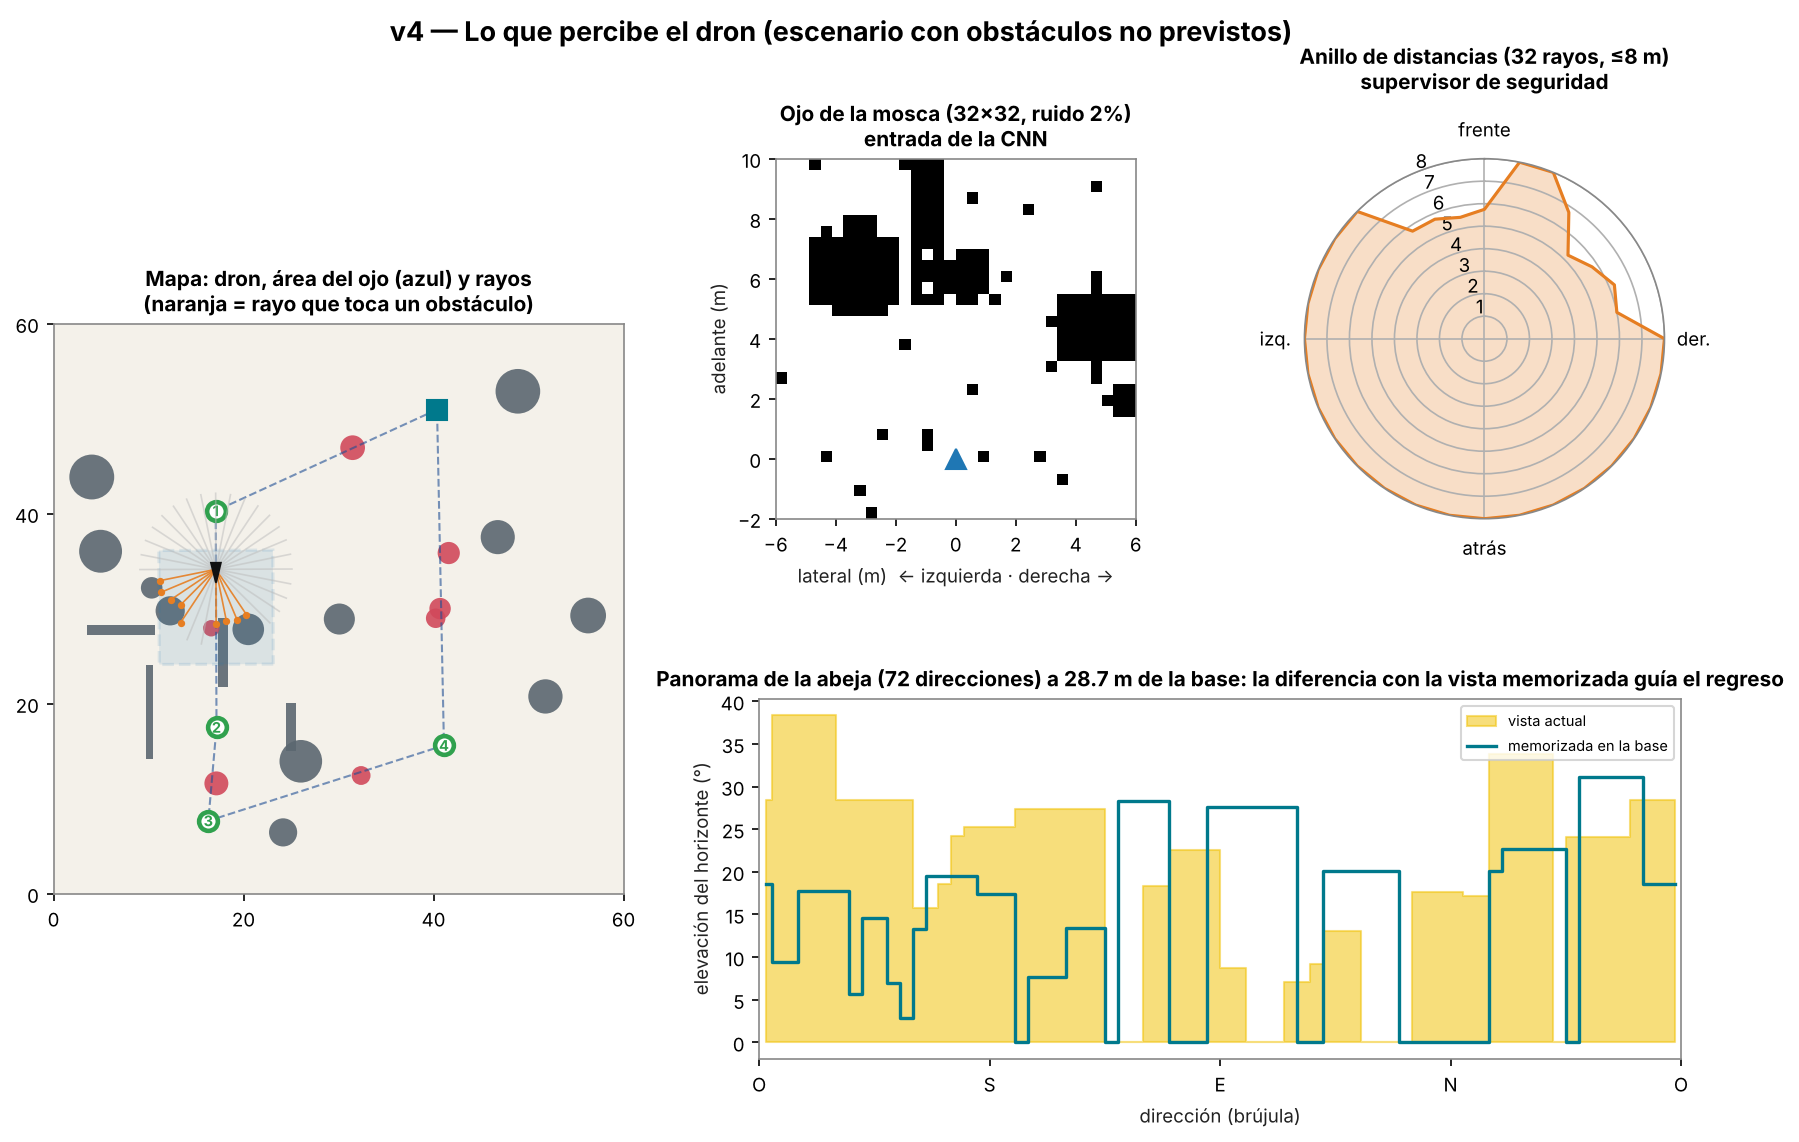
\includegraphics[width=0.9\textwidth]{v4_sensores}
\caption{Lo que percibe el dron: área del ojo y rayos sobre el mapa, ojo de la mosca (entrada
de la CNN), anillo de distancias (supervisor) y panorámica de la abeja.}
\label{fig:sensores}
\end{figure*}

\begin{figure*}[t]
\centering
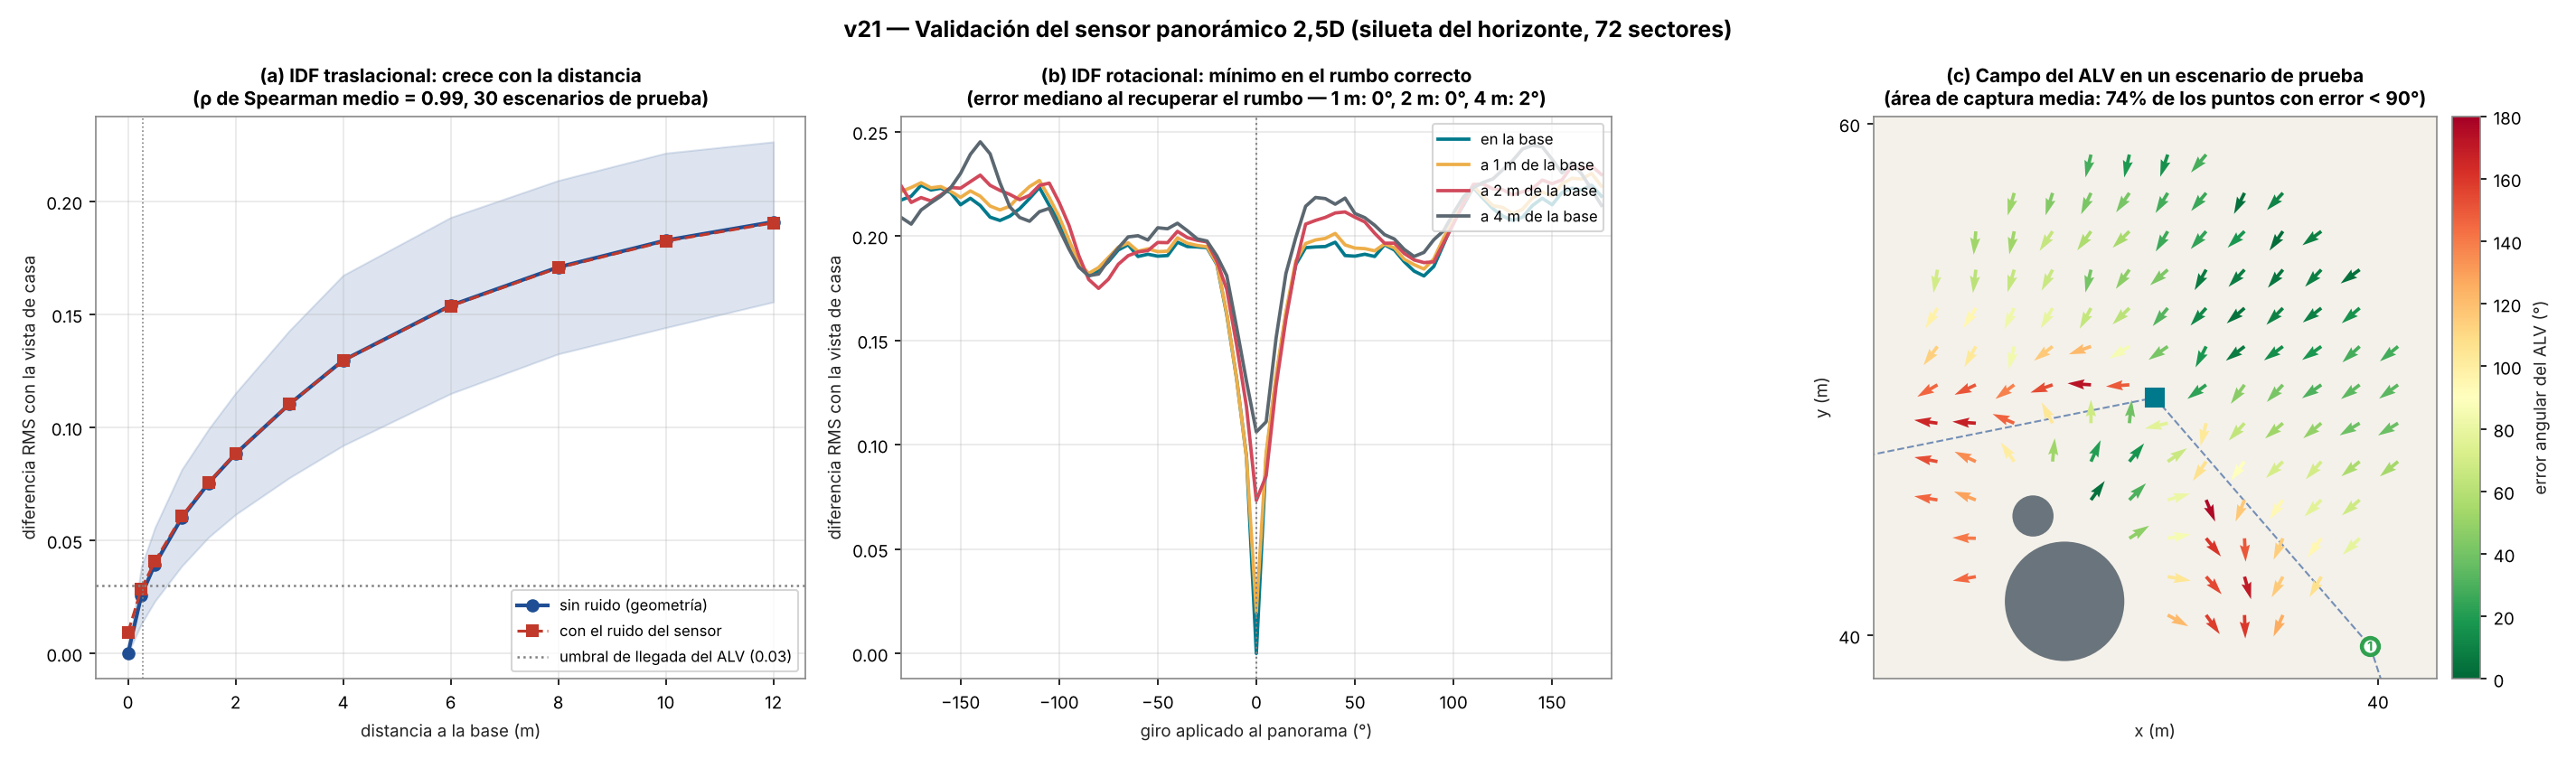
\includegraphics[width=\textwidth]{v21_validacion_sensor}
\caption{Validación del sensor panorámico 2.5D en escenarios de prueba: (a) IDF traslacional
(media $\pm$ d.e.) sin ruido y con el ruido del sensor; (b) IDF rotacional en la base y a 1,
2 y 4\,m; (c) campo del ALV coloreado por su error angular.}
\label{fig:sensor}
\end{figure*}
